\documentclass[12pt]{article}
\usepackage[utf8]{inputenc}

%%% I added a few packages. This next one allows you to set the margins.
\usepackage[top=.5in,bottom=1in,right=.75in,left=.75in]{geometry}
\usepackage{multicol}
%\usepackage{newspaper}
\setlength{\columnsep}{1cm}
\usepackage{blindtext}
\usepackage{varwidth}

%%% This one does boxes in a really nice way.
\usepackage{tcolorbox}
\usepackage{mdframed}
\usepackage{minibox}
\usepackage{graphicx}
\graphicspath{ {./images/} }
\usepackage{epstopdf}
  \epstopdfDeclareGraphicsRule{.pdf}{png}{.png}{convert #1 \OutputFile}
  \DeclareGraphicsExtensions{.png,.pdf}
\usepackage{hyperref}
\hypersetup{
    colorlinks=true,
    linkcolor=blue,
    filecolor=magenta,      
    urlcolor=cyan,
    pdftitle={MSCSMess},
    pdfpagemode=FullScreen,
    }
\urlstyle{same}
 \usepackage{fix-cm}
 \usepackage{soul}
 \usepackage{graphicx}
 \usepackage{multicol}


\newcommand{\ds}{\displaystyle}
\newcommand{\ZZ}{\mathbb{Z}}
\newcommand{\QQ}{\mathbb{Q}}
\newcommand{\RR}{\mathbb{R}}
\newcommand{\CC}{\mathbb{C}}
\newcommand{\FF}{\mathbb{F}}
\newcommand{\xx}{\mathbf{x}}
\newcommand{\uu}{\mathbf{u}}
\newcommand{\vv}{\mathbf{v}}

\newcommand{\bolder}{\textbf}
 
 
\title{\fontsize{60}{70}\selectfont {\bf {MSCS} 
\includegraphics[scale=.3]{images/OleLion.png} {Mess}}}
\author{Department of Mathematics, Statistics, and Computer Science \\ St.\@ Olaf College, Northfield, MN 55057 \vspace{-2ex}} 
\date{\today\, $|$ Volume 54, No.\@ 24 \line(1,0){500}}


\begin{document}

\maketitle \vspace{-1cm}
\begin{center}
Happy Friyay! Check out some of the cool events that are coming up and of course have a beautiful start to May!

\end{center}

 \begin{multicols}{2}


\begin{tcolorbox}[colback=white, colframe=black]
    \begin{center}
    \title{{\large \bolder{NSM Honors Day Poster Session!}}}
    \end{center}
\end{tcolorbox}

HAPPENING TODAY! Join us for this year’s NSM Honors Day Poster Session! We invite anyone who has completed research (on or off campus) to present their work. The event is open to everyone, and snacks and beverages will be served. Please see the \href{https://wp.stolaf.edu/physics/honorsdaypostersession_sci_math/} {NSM Honors Day Poster Session website} for more information! 

\begin{tcolorbox}[colback=white, colframe=black]
    \begin{center}
    \title{{\large \bolder{Math Across the Cannon}}}
    \end{center}
\end{tcolorbox}
Join us for Math Across the Cannon on May 4-5 featuring Professor Jennifer Hill from NYU. On Monday, May 4, she will speak at St. Olaf in Regents Hall 150, with a reception at 3:30pm and lecture at 4:00pm, discussing the challenges of multiple comparisons in statistical research. On Tuesday, May 5, she will present at Carleton College in the Weitz Cinema at 6:00pm, exploring the promises and limitations of artificial intelligence in her talk about ChatGPT. This is a great opportunity to hear a talk from an excellent speaker, and network with some of our Carleton friends!

\begin{tcolorbox}[colback=white, colframe=black]
    \begin{center}
    \title{{\large \bolder{Bunnies on campus!}}}
    \end{center}
\end{tcolorbox}
Women in STEM is hosting a fun event to celebrate the school year and destress before finals! They will have baby bunnies from Windy Willow Farm in the lawn between Regents and Old Main from 3-4pm on Wednesday May 6!


\begin{tcolorbox}[colback=white, colframe=black]
    \begin{center}
    \title{{\large \bolder{MSCS Senior Banquet}}}
    \end{center}
\end{tcolorbox}

MSCS graduating seniors are invited to attend this year's Senior Banquet on May 7th at 5:30pm. Please RSVP using \href{https://docs.google.com/forms/d/e/1FAIpQLScgOKI8CBUjdAlBOWogwo_QmVcTVVHmFHDOw5-bzeL7vT30CQ/viewform}{this link} by Tuesday, April 28th. 

\begin{tcolorbox}[colback=white, colframe=black]
    \begin{center}
    \title{{\large \bolder{Computer Science Showcase}}}
    \end{center}
\end{tcolorbox}

Come see what your fellow Oles have been building! The Computer Science Showcase is on Monday, May 11th at 3:30pm in the Buntrock Commons Sun Ballroom. CS students will present their year-long projects, and there will be snacks, good vibes, and prizes up for grabs. Want to show off your own project? Scan the QR code on the poster or reach out to Prof. Leeson (leeson2@stolaf.edu) to sign up.

\begin{tcolorbox}[colback=white, colframe=black]
    \begin{center}
    \title{{\large \bolder{Have you done math research?
    }}}
    \end{center}
\end{tcolorbox}
Professor Dietz edits an annual volume of mathematics research papers written by students, whether the research was supervised by a St. Olaf faculty member or not. If you've done something original in an REU, DUR, IR/IS between about May 2025 and now, please email dietz@stolaf.edu. 

\begin{tcolorbox}[colback=white, colframe=black]
    \begin{center}
    \title{{\large \bolder{Problem Solving Group}}}
    \end{center}
\end{tcolorbox}
The Math Problem Solving Group meets weekly to have fun, solve math problems, eat candy, and prepare for upcoming math contests. Meetings are Thursdays from 11:30 am - 12:30 pm, in RNS 207 (the Center for Interdisciplinary Research room). Everyone is welcome, regardless of prior experience in mathematics or math contests!


\end{multicols} \vspace{3cm} 


\begin{center}
    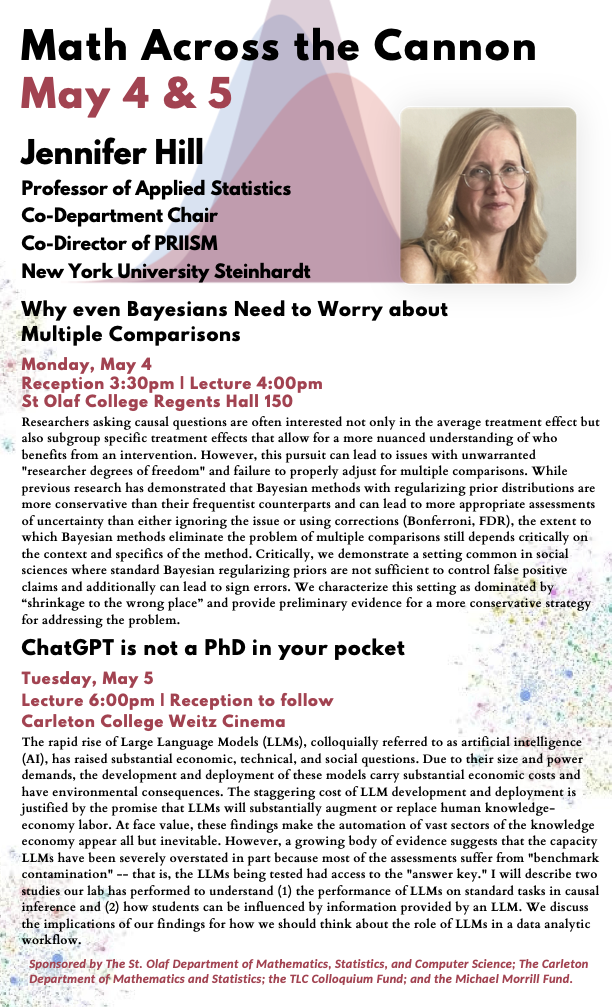
\includegraphics[height=1.00\textheight]{images/Math Across the Cannon (8.5 x 14 in)-1.png}
\end{center}

\begin{center}
    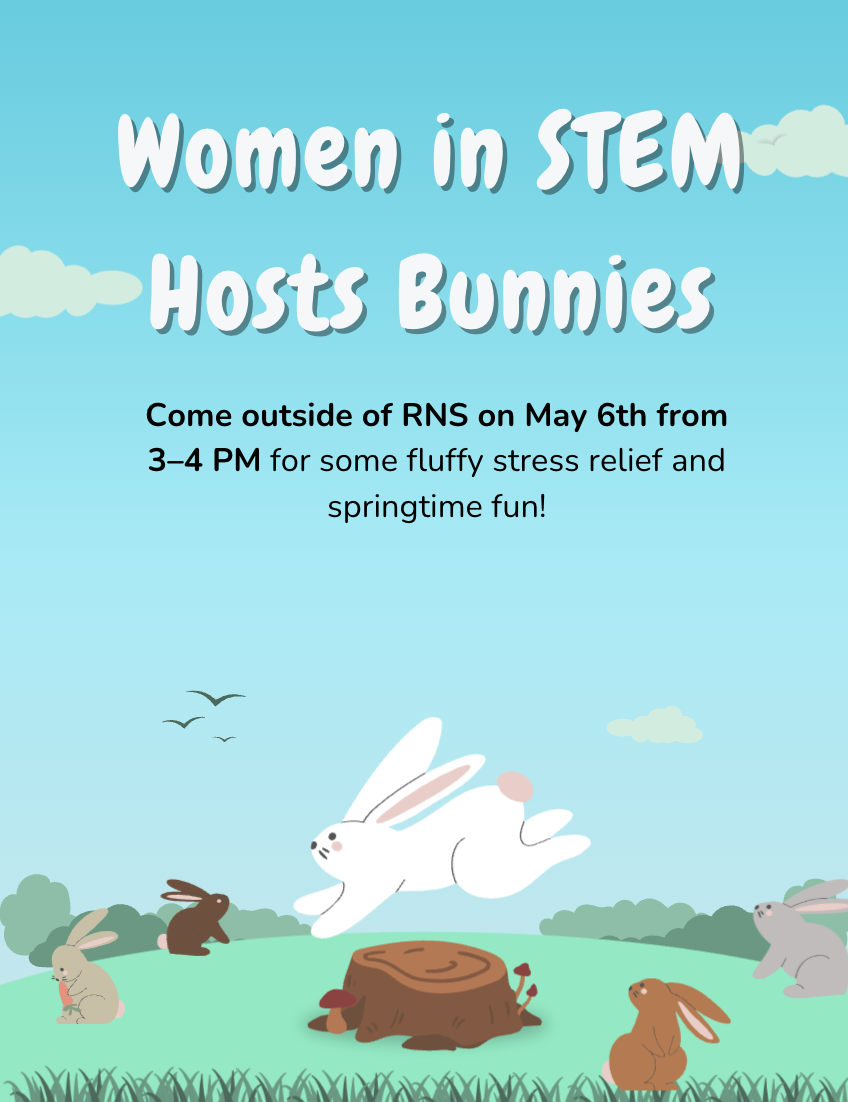
\includegraphics[height=0.95\textheight]{images/BunniesBeforeFinals - WIS.png}
\end{center}

\begin{center}
    
\includegraphics[height=0.95\textheight]{Senior Banquet 2026.png}
\end{center}



\begin{center}
    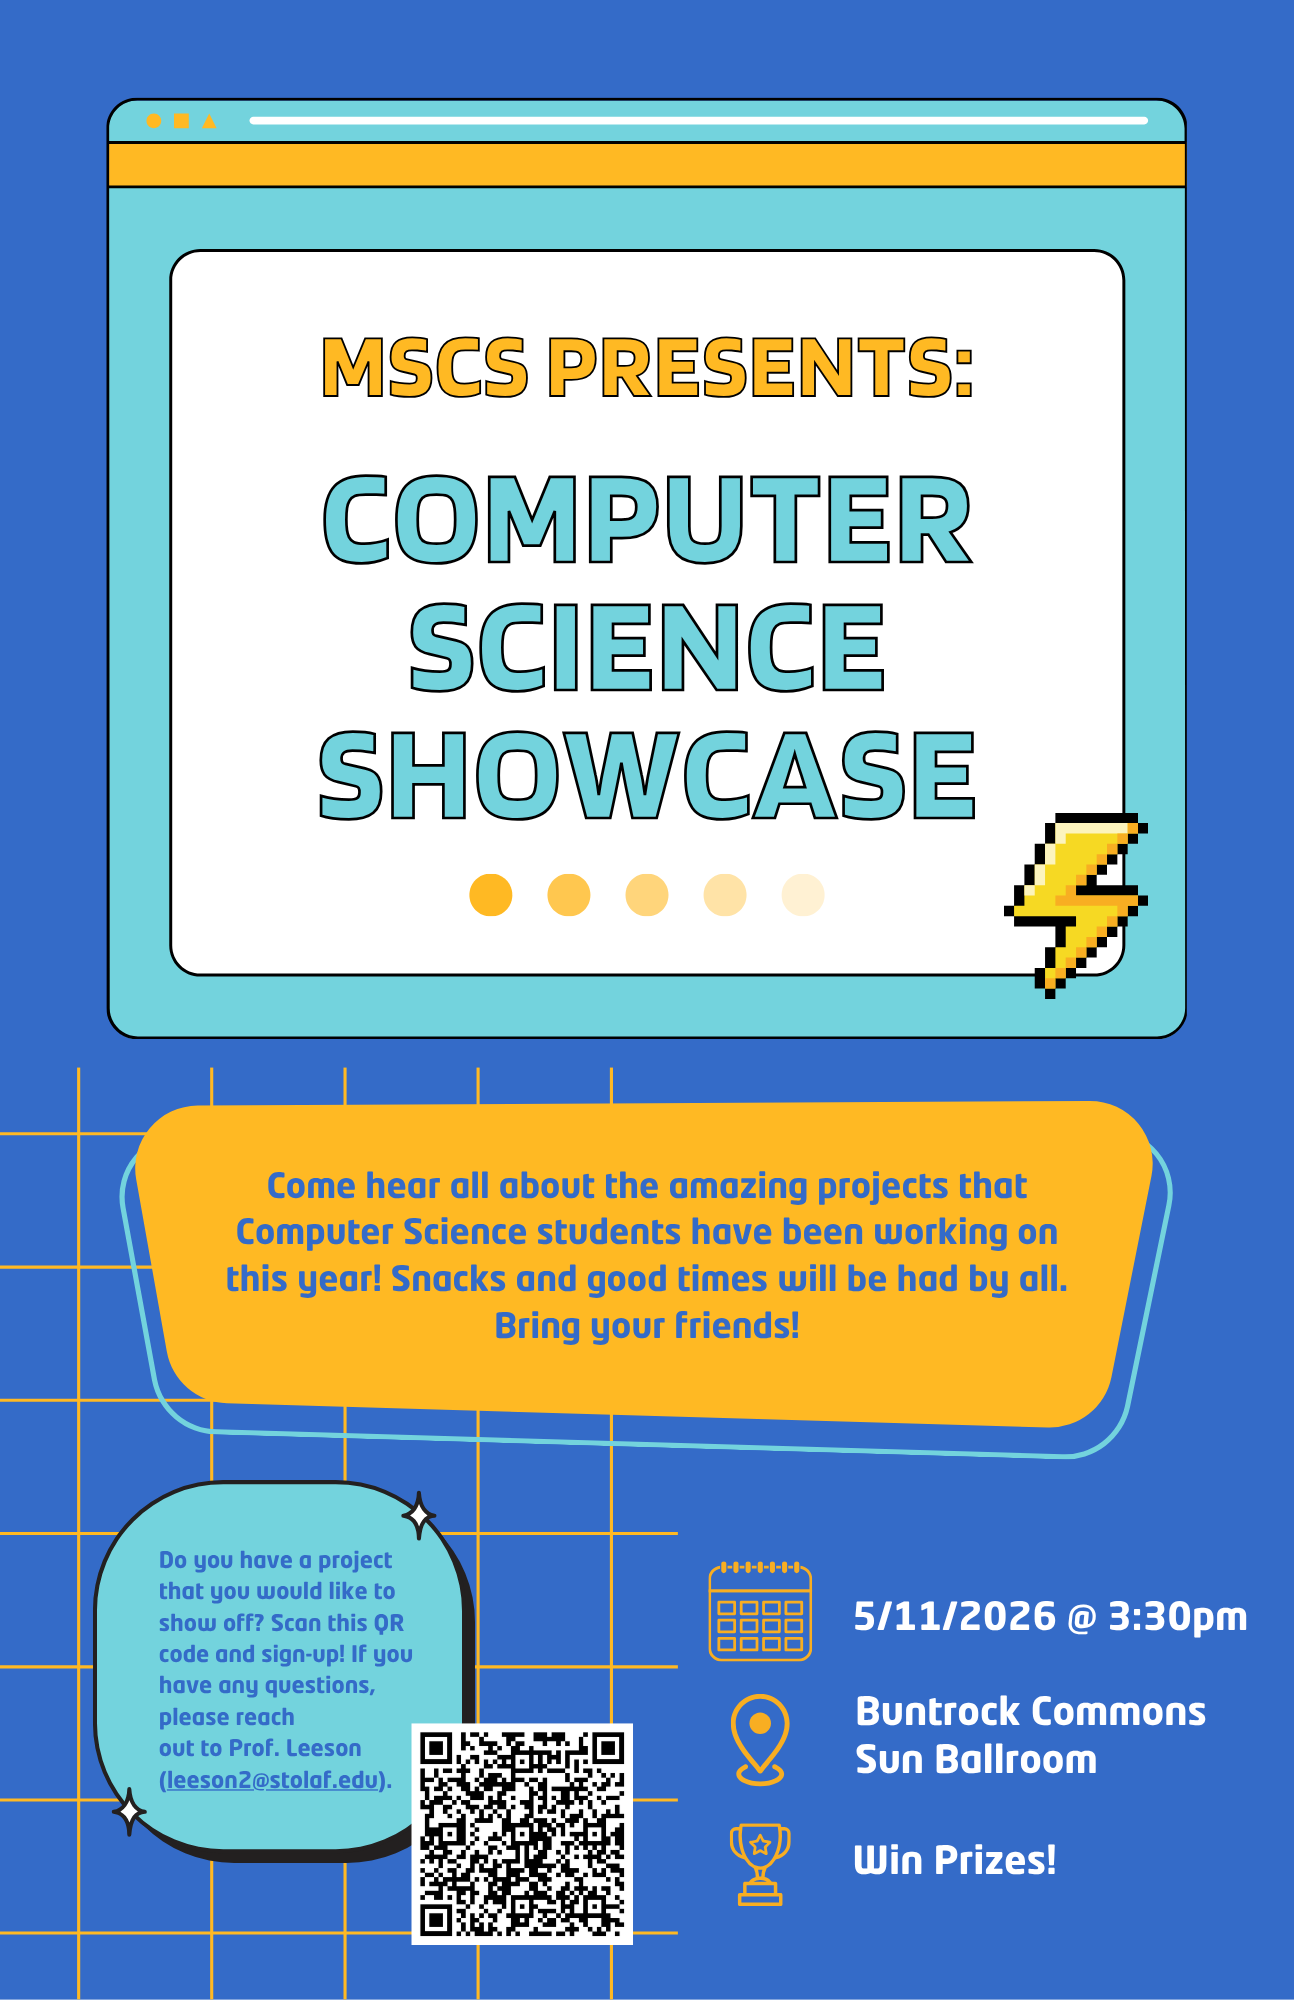
\includegraphics[height=0.95\textheight]{images/Computer Science Showcase (1).png}
\end{center}


\begin{center}
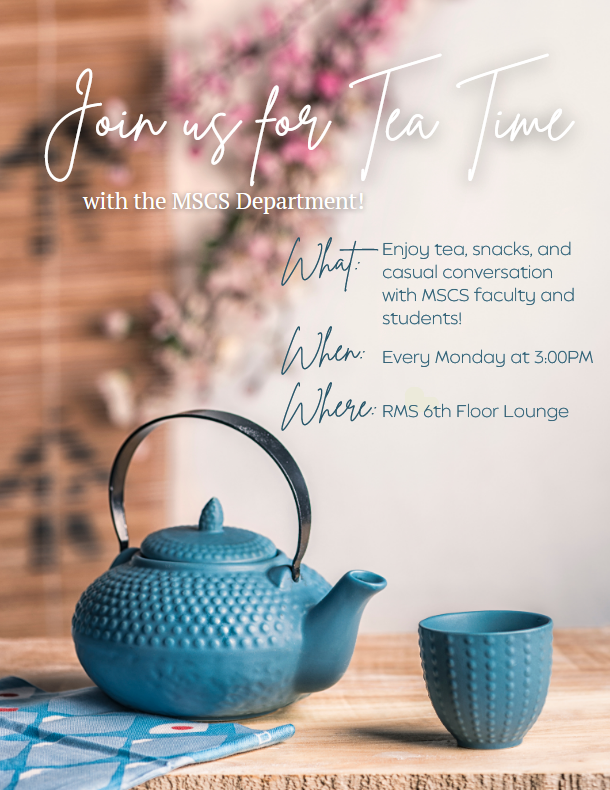
\includegraphics[width=0.9\textwidth]{images/Tea Time Poster.png}
\end{center}

\noindent{To submit an article, event, or anything else for publication in the Mess, email messeditor@stolaf.edu. Visit \href{https://wp.stolaf.edu/mscs/mscs-mess/}{http://wp.stolaf.edu/mscs/mscs-mess/} for a digital archive of previous MSCS Mess issues.}\\
	
\hfill Nima Dahir, Editor
	
\hfill Kyle Salois, Faculty Advisor


 

\end{document}